\documentclass[conference,letterpaper,10pt]{IEEEtran}
\IEEEoverridecommandlockouts
\usepackage[T1]{fontenc}
\usepackage{lmodern}
\usepackage{amsmath,amssymb,graphicx,booktabs,array,xcolor}
\usepackage{url}
\usepackage{microtype}
\usepackage{tikz}
\usetikzlibrary{arrows.meta,positioning,shapes.geometric}
\usepackage[hidelinks]{hyperref}
\renewcommand{\arraystretch}{1.12}
\title{Progress Review: Vision-Guided Rendezvous and Magnetic Docking with a Differential-Drive Ground Robot}
\author{\IEEEauthorblockN{Zein Barakat, Justin Puran, Santiago Calderon-Rueda, and Ryan Flowers}
\IEEEauthorblockA{EGN 4060C -- Introduction to Robotics\\University of Central Florida, Orlando, Florida, USA\\November 2026}}
\begin{document}
\maketitle
\begin{abstract}
This report documents the progress of a low-cost ground-robot testbed for spacecraft-inspired rendezvous, proximity operations, and docking (RPOD). A Pololu Romi differential-drive robot serves as the chaser; a stationary, AprilTag-equipped magnetic interface serves as the target. The team has completed the reported hardware assembly, soldering, and wiring, established Raspberry Pi--Arduino communications, demonstrated AprilTag detection and live camera-relative pose estimates, and collected 48 checkerboard images for camera calibration. The constrained camera model produced an RMS reprojection error of 0.864 pixels, but metric pose accuracy has not yet been validated against measured distances. The remaining work is hardware-in-the-loop integration, motor and sensor characterization, estimation, trajectory generation, feedback control, and repeated docking trials. Dynamic-target docking is proposed as an optional extension after the stationary baseline is reliable.
\end{abstract}
\begin{IEEEkeywords}
robotics, autonomous docking, AprilTag, differential drive, camera calibration, state estimation, guidance and control
\end{IEEEkeywords}

\section{Problem and Project Objective}
Autonomous rendezvous and docking require a vehicle to locate a target, estimate relative pose, plan an admissible approach, correct its motion using feedback, and make controlled physical contact. Although spacecraft RPOD is the motivation, this project isolates analogous perception, navigation, guidance, and control concepts on a two-dimensional ground robot rather than reproducing orbital dynamics. The chaser begins at a variable pose and must reach a fixed docking interface with the correct final position, heading, and low approach speed. The project is intended to demonstrate feedback-controlled autonomy, not merely a timed forward-driving maneuver.

The proposed mission has five phases: target acquisition; travel to a pre-docking pose; heading alignment; decelerated final approach; and magnetic contact. A curved path is desirable when the initial heading is not aligned with the port, but trajectory optimality must be defined by explicit objectives and constraints, not by the presence of curvature alone. The baseline is \emph{stationary-target} docking; tracking or docking with a moving target is a stretch goal.

\section{System Design}
\subsection{Hardware and Electrical Architecture}
The chaser uses a Pololu Romi chassis with two DC gearmotors and quadrature wheel encoders, an Arducam IMX219 camera, an MPU-6050 inertial measurement unit (IMU), an Arduino Nano, a TB6612FNG dual H-bridge, and a Raspberry Pi Zero 2 W. Mechanical construction, soldering, mounting, and interconnection are reported complete, with functional motor and telemetry verification still outstanding. The Raspberry Pi executes image processing and high-level robotics software; the Arduino is assigned encoder acquisition, motor actuation, and low-level control. The Pi is supplied separately by a regulated 5 V USB source; motor-battery voltage, grounds, and current handling require measured verification before powered drivetrain trials.

The docking station will provide a single, known magnetic contact point and a mechanically defined approach direction. An AprilTag attached rigidly near the interface serves as the visual reference. A future docking fixture may use guide surfaces for passive final alignment; its geometry and holding force remain to be tested.

\subsection{Software and GNC Information Flow}
The intended closed loop is illustrated in Fig.~\ref{fig:architecture}. Camera measurements provide a target pose relative to the camera. Encoder odometry and IMU yaw-rate measurements will support robot-state prediction; camera-to-robot transformations will place measurements into compatible reference frames. An extended Kalman filter (EKF) is planned to estimate the planar state $\mathbf{x}=[x\;y\;\theta]^T$ and its uncertainty. A guidance layer will generate a pre-docking pose and speed/heading references, and wheel-speed PID loops will command the motors. These are \emph{planned} integrated functions, not yet validated subsystems.

\begin{figure}[t]
\centering
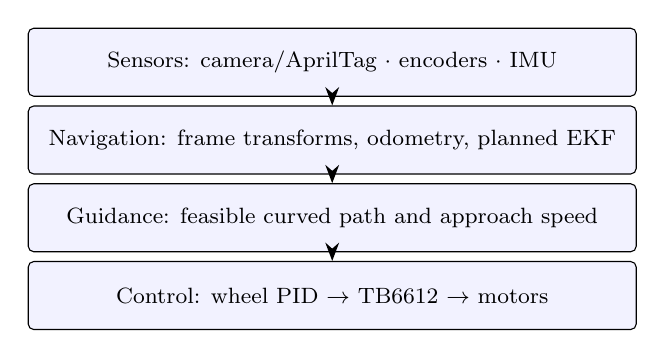
\begin{tikzpicture}[>=Stealth, node distance=1.1mm, font=\footnotesize, every node/.style={align=center}]
\node[draw,rounded corners=2pt,fill=blue!5,minimum width=3.04in,minimum height=.34in] (s) {Sensors: camera/AprilTag $\cdot$ encoders $\cdot$ IMU};
\node[draw,rounded corners=2pt,fill=blue!5,minimum width=3.04in,minimum height=.34in,below=of s] (n) {Navigation: frame transforms, odometry, planned EKF};
\node[draw,rounded corners=2pt,fill=blue!5,minimum width=3.04in,minimum height=.34in,below=of n] (g) {Guidance: feasible curved path and approach speed};
\node[draw,rounded corners=2pt,fill=blue!5,minimum width=3.04in,minimum height=.34in,below=of g] (c) {Control: wheel PID $\rightarrow$ TB6612 $\rightarrow$ motors};
\draw[->,thick] (s)--(n);\draw[->,thick] (n)--(g);\draw[->,thick] (g)--(c);
\end{tikzpicture}
\caption{Proposed closed-loop architecture. Hardware and the isolated vision/serial tests exist; EKF, guidance, and wheel PID remain integration tasks.}
\label{fig:architecture}
\end{figure}

\section{Progress and Demonstrated Results}
\subsection{Assembly and Processor Communications}
The hardware build has progressed through mechanical assembly, soldering, and wiring. The Arduino Nano was successfully programmed, and USB serial communication was independently tested using a \texttt{PING} / \texttt{PONG} exchange. Firmware also parses \texttt{SET}, \texttt{STATUS}, and \texttt{STOP} messages and includes a command-timeout watchdog. The \texttt{SET} values are command targets; this test does \emph{not} demonstrate closed-loop motor speed or actual wheel response. Successful Pi-to-Nano serial operation on the final assembled system, motor polarity, encoder counts, IMU axes, and telemetry timing still require verification.

\subsection{Vision Pipeline and Camera Calibration}
The Pi Zero 2 W successfully captured images from its IMX219 camera using libcamera/Picamera2. OpenCV detected a printed AprilTag from a live camera image, identified tag ID 0, and returned its pixel center and image corners. A live browser dashboard subsequently displayed camera-relative translation, estimated range, bearing, and marker orientation using a Perspective-n-Point (PnP) calculation \cite{olson2011,opencvcalib}. Fig.~\ref{fig:dashboard} shows an example recorded output; it illustrates functioning detection and pose computation, \emph{not independently verified dimensional accuracy}.

\begin{figure}[t]
\centering
\includegraphics[width=\columnwidth]{live_tag_dashboard.png}
\caption{Team camera output: AprilTag ID 0, detected corner outline, and live relative-pose readout. The displayed range is an estimator output, not a ground-truth distance measurement.}
\label{fig:dashboard}
\end{figure}

A 9-by-6 inner-corner checkerboard (nominal 18 mm squares) was photographed at 640$\times$480 resolution over 48 usable views. The original five-coefficient calibration achieved 0.769-pixel RMS reprojection error but estimated an off-center principal point and extreme higher-order distortion. A constrained model fixed the principal point near the image center and estimated fewer distortion terms, giving 0.864-pixel RMS with
\begin{equation}
K\approx\begin{bmatrix}1487.60&0&319.5\\0&1488.53&239.5\\0&0&1\end{bmatrix},\quad k_1\approx0.6584.
\label{eq:intrinsics}
\end{equation}
The lower RMS of the unconstrained fit does not establish superior physical accuracy. Both models require validation at measured distances and viewpoints; the printed tag size must also be checked because an incorrect physical scale directly biases PnP translation.

\begin{table}[t]
\centering\caption{Progress status at the review date}\label{tab:status}
\footnotesize
\begin{tabular}{p{1.25in}p{1.72in}}
\toprule
\textbf{Activity} & \textbf{Status / evidence}\\\midrule
Mechanical/electrical build & Assembly, soldering, wiring reported complete; power checks pending\\
Arduino program and protocol & Flash, PING/PONG, parser, watchdog tested\\
Vision acquisition / detection & IMX219 capture and AprilTag ID 0 demonstrated\\
Camera calibration & 48 views; 0.769 px original / 0.864 px constrained RMS\\
Metric pose accuracy & Pose dashboard operating; tape-measured validation pending\\
Motor, encoder, IMU, EKF, docking & End-to-end functionality not yet established\\\bottomrule
\end{tabular}
\end{table}

\section{Integration and Evaluation Plan}
\subsection{Gated Development Sequence}
Work is organized into four tentative stages. \textbf{(1) Electrical and telemetry:} check all supply rails and polarities under load; verify USB communications, encoder quadrature direction/counts, IMU orientation, serial packet timing, and a safe stop response. \textbf{(2) Actuation and odometry:} conduct individual motor tests at low duty cycle; determine wheel-radius and track-width calibrations; measure RPM step responses; tune left/right PID and quantify repeatability. \textbf{(3) Navigation and guidance:} validate AprilTag ranges and lateral offsets against physical measurements; measure camera-to-body extrinsics; implement differential-drive propagation, then fuse available sensor measurements; plan feasible curved approaches. \textbf{(4) Docking trials:} construct and locate the magnet/guide fixture, define a staging point and low-speed contact rule, and run repeated trials from different initial poses. Each stage must pass before progressing to physical contact tests.

For planar differential drive, incremental encoder displacement provides the nominal motion model
\begin{align}
\Delta s&=\frac{\Delta s_R+\Delta s_L}{2}, &
\Delta\theta&=\frac{\Delta s_R-\Delta s_L}{b},\nonumber\\[-2pt]
\Delta x&\approx\Delta s\cos\!\left(\theta+\frac{\Delta\theta}{2}\right), &
\Delta y&\approx\Delta s\sin\!\left(\theta+\frac{\Delta\theta}{2}\right),
\label{eq:odom}
\end{align}
where $b$ is wheel separation. This model will be checked against measured trajectories before it is used in an EKF. The planned final docking error is measured at the physical contact reference, not merely at the AprilTag center.

\subsection{Performance Metrics and Expected Outcomes}
The team will report independent measurements rather than assuming success from a visual demo. Table~\ref{tab:metrics} defines the planned test outputs. A successful baseline demonstration would show stable visual target acquisition, repeatable low-speed motion, bounded terminal pose error, and physical magnet engagement from multiple starting configurations. Target thresholds will be selected after characterizing the guide geometry and sensor uncertainty, rather than asserted prematurely.

\begin{table}[t]
\centering\caption{Planned quantitative validation}\label{tab:metrics}
\footnotesize
\begin{tabular}{p{1.32in}p{1.65in}}
\toprule
\textbf{Metric} & \textbf{Measurement protocol}\\\midrule
Camera depth error & $|\hat Z-Z_{\mathrm{tape}}|$ at multiple measured depths; repeatability and bias\\
Wheel-speed control & RPM reference vs. measured RPM; rise time, overshoot, steady-state error\\
Odometry / path error & Position and heading drift; cross-track RMSE on known paths\\
Terminal docking accuracy & Magnet-to-port position and heading error at stop/contact\\
Docking reliability & Successful contacts / total trials over varied initial poses\\
Time and safety & Time to dock; contact speed; loss-of-tag and watchdog response\\\bottomrule
\end{tabular}
\end{table}

\section{Stretch Goal: Curved Rendezvous with a Moving Target}
A moving docking platform would extend the baseline only after adequate stationary accuracy, camera update rate, and stop behavior are demonstrated. The existing forward-facing camera can track a moving AprilTag, so LiDAR is not a prerequisite for a controlled, visible target. One or more additional, uniquely identified tags could be fixed to angled faces of the target, with each tag's surveyed transform to the \emph{same} docking-port reference. For visible tag $i$,
\begin{equation}
{}^{C}T_D={}^CT_{T_i}\;{}^{T_i}T_D,
\label{eq:tag}
\end{equation}
where ${}^{C}T_{T_i}$ is visually estimated and ${}^{T_i}T_D$ is determined from the rigid mounting geometry. This allows different tag IDs to describe one docking destination. Temporary occlusions would require state prediction with increasing uncertainty and a slow/stop policy if the target remains unobserved.

Rather than prescribing a circular track, a future planner would minimize a weighted combination of terminal position, heading and relative-speed errors, travel time, control effort, and tag visibility, subject to differential-drive curvature, motor limits, and physical collision constraints. A smooth curved approach can then transition into a short, nearly straight final contact segment. Predictive guidance for a moving dock would additionally require estimating target velocity and replanning. These features are \emph{proposed research directions}, not completed results.

\section{Conclusion}
The project has advanced from a conceptual RPOD architecture to a wired, assembled Romi platform with demonstrated camera acquisition, AprilTag identification, live pose computation, Arduino command parsing, and a 48-image camera calibration dataset. The critical work now is to verify electrical and sensor interfaces, characterize motion, validate metric pose estimates, close the feedback loop, and demonstrate repeatable magnetic docking. The proposed evaluation will determine whether the team can justify more ambitious curved and moving-target rendezvous experiments.

\begin{thebibliography}{00}
\bibitem{olson2011} E. Olson, ``AprilTag: A robust and flexible visual fiducial system,'' in \emph{Proc. IEEE Int. Conf. Robotics and Automation (ICRA)}, 2011, pp. 3400--3407.
\bibitem{opencvcalib} OpenCV, ``Camera calibration and 3D reconstruction,'' \emph{OpenCV Documentation}. [Online]. Available: \url{https://docs.opencv.org/4.x/d9/d0c/group__calib3d.html}
\bibitem{romi} Pololu, ``Romi chassis kit -- black,'' product no. 3500. [Online]. Available: \url{https://www.pololu.com/product/3500}
\bibitem{thrun} S. Thrun, W. Burgard, and D. Fox, \emph{Probabilistic Robotics}. Cambridge, MA, USA: MIT Press, 2005.
\end{thebibliography}
\end{document}
